\documentclass{beamer}
\usepackage[utf8]{inputenc}
\usepackage{algorithmic}
\usepackage{algorithm}
\usepackage{amsfonts}
\usepackage{amssymb}
\usepackage{courier}
\usepackage{graphicx}
\usepackage{listings}
\usepackage{mathtools}
\usepackage[font={small}, labelfont={color=black}]{caption}
\usetheme{Rochester}

\usefonttheme[onlymath]{serif}
\beamertemplatenavigationsymbolsempty
\title{\LARGE{Evolving Behaviour Trees}\\
       \small{\emph{Learning Behaviour in Top-Down Shooter}}}
\author{\vspace{2ex}\\\textbf{Martin Estgren} \;\,\;\;\,\,
        \texttt{<mares480@student.liu.se>} \\
        \textbf{Erik S. V. Jansson}\;
        \texttt{<erija578@student.liu.se>} \\~\\
        {Artificial Intelligence for Interactive Media}\\
        {ITN Linköping University (LiTH),\, Sweden}}

\lstset{
    escapeinside={<@}{@>},
    basicstyle=\tiny\ttfamily,
    breakatwhitespace = false,
    breaklines = true,
    captionpos = b,
    keepspaces = true,
    language = Java,
    showspaces = false,
    showstringspaces = false,
    frame = tb,
    aboveskip = 10pt,
    belowskip = 10pt,
    numbers = left,
    numbersep = 3pt
}

\setbeamerfont{bibliography item}{size=\tiny}
\setbeamerfont{bibliography entry author}{size=\tiny}
\setbeamerfont{bibliography entry title}{size=\tiny}
\setbeamerfont{bibliography entry location}{size=\tiny}
\setbeamerfont{bibliography entry note}{size=\tiny}
\setbeamertemplate{footline}[frame number]
\begin{document}
    \frame{\titlepage}

    \frame{\frametitle{Outline}
        \begin{enumerate}
            \item{Motivation}
            \item{Techniques}

                \begin{itemize}
                    \item{Behaviour Trees}
                    \item{Path Finding w/ A*}
                    \item{Genetic Programming}
                \end{itemize}

            \item{Implementation}

            \item{Demonstration}

                \begin{itemize}
                    \item{Pre-Defined\, Behaviour Trees}
                    \item{Behaviour Tree GP Evolution}
                \end{itemize}

            \item{Results}

            \item{Discussion}
        \end{enumerate}
    }

    \frame{\frametitle{Motivation}
        Goal: create a fun an challenging adversarial bot to play against.\\
        \begin{itemize}
            \item{Some game with a sufficiently complex environment: Quake}
            \item{Represent knowledge and decision making:\, Behaviour Trees}
            \item{Interesting and dynamic behaviours: Genetic Programing}
        \end{itemize}
    }

    \frame{\frametitle{Techniques} \framesubtitle{Behaviour Trees}
        Models the decision-making process by using trees composed of \emph{control-flow nodes} and \emph{execution nodes}.
        \begin{figure}
            \centering
            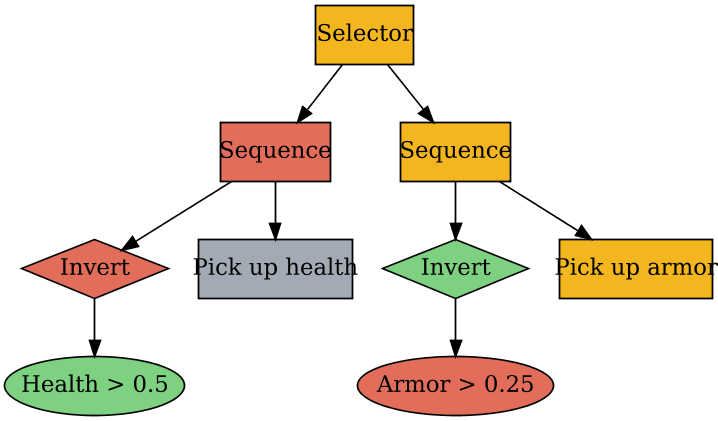
\includegraphics[width=0.8\textwidth]{share/bt.png}
        \end{figure}
    }

    \frame{\frametitle{Techniques} \framesubtitle{A* Path Finding}
        Heuristic-based graph-traversal search algorithm.

        \begin{itemize}
            \item{\textbf{Path cost:} cost \(g(n)\) of reaching the current node \(n\).}
            \item{\textbf{Heuristic:} estimated cost \(h(n)\) to reach goal.}
            \item{Expand the nodes with the lowest \(f(n) = g(n) + h(n)\)}
        \end{itemize}

        \begin{figure}
            \centering
            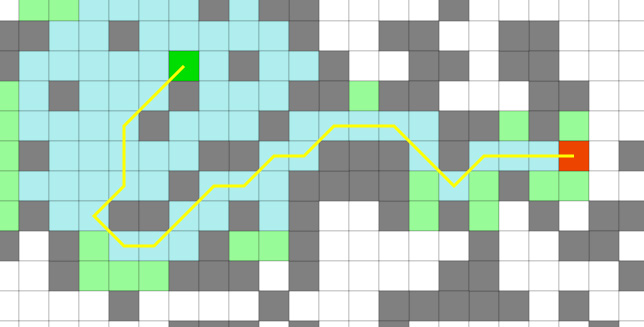
\includegraphics[width=0.6\textwidth]{share/path_finding.jpg}
        \end{figure}
    }

    \frame{\frametitle{Techniques} \framesubtitle{Genetic Programming}
        \begin{enumerate}
            \item{\textbf{Selection:} technique for determining future \emph{populations} by picking individuals by using a \emph{fitness function}.}
            \item{\textbf{Crossover:} pick \emph{individuals} in the population and produce \emph{offspring} by mixing a subset of their features.}
            \item{\textbf{Mutation:} alter individuals' properties randomly to diversify the population to potentially get better behaviours.}
        \end{enumerate}
        \begin{itemize}
            \item{\(\rightarrow\) very similar to the \emph{natural selection} process of evolution.}
        \end{itemize}
    }

    \frame{\frametitle{Implementation}
        \begin{itemize}
            \item{\textbf{Behaviour trees:} we've implemented high-level actions e.g. attack ``player'' to limit the structural complexity of the tree.}
            \item{\textbf{Path finding:} \emph{waypoint-based} navigation with \emph{Euclidean distance} as heuristic. Other player's field of view affects path cost (also called an \emph{influence map}): avoid player line of sight.}
            \item{\textbf{Genetic programming:} selection of individuals proportional to fitness, we mutate the structure and parameters of the tree and then cross them over by swapping pairs of sub-trees.}
        \end{itemize}
    }

    \frame{\frametitle{Demonstration}
        \begin{itemize}
            \item{Base game}
            \item{Behaviour tree}
            \item{Bot vs bot}
            \item{Tree evolution}
            \item{Natural selection}
        \end{itemize}
    }

    \frame{\frametitle{Results}
    }

    \frame{\frametitle{Discussion}
        We've implemented a top-down shooter where bot decisions are made with \emph{behaviour trees}, controlled using \emph{A* path finding} and optimized using \emph{genetic programming}. All from scratch in Java.

        \begin{itemize}
            \item{\textbf{Our goals:} create a fun an challenging bot to play against.}
            \item{\textbf{What went right:} game is fun to play, behaviour trees allows to easily make complex behaviours, genetic programming creates interesting and new behaviours and robust path finding, the component-entity-system.}
            \item{\textbf{What went wrong:} genetic programming didn't work at first, many bugs related to physics and the crunch-time week.}
            \item{\textbf{Improvements:} better selection heuristic, more interesting actions, adversarial resource competition.}
        \end{itemize}
    }

    \frame{\frametitle{Questions?}}
    \frame{\frametitle{Bibliography}
        \nocite{*}
        \bibliographystyle{alpha}
        \bibliography{slides}
    }
\end{document}
